%%%% Small single column format
\documentclass[anonymous=false, %
               format=acmsmall, %
               review=true, %
               screen=true, %
               nonacm=true]{acmart}

\usepackage[ruled]{algorithm2e}
%\usepackage{parskip}
\usepackage{subcaption}
\usepackage{fontawesome}
\usepackage{footnote}
\makesavenoteenv{tabular}
\makesavenoteenv{table}
\usepackage{tabularx}

\urlstyle{tt}
\citestyle{acmauthoryear}

\begin{document}

\title{{ArviZ}: backend agnostic exploratory analysis of
{Bayesian} models in {Python}}

\author{Oriol Abril}
\orcid{0000-0002-1847-9481} % chktex 8
\affiliation{%
  \institution{Universitat Pompeu Fabra}
  % \department{Department of Brain and Cognitive Sciences}
  %\streetaddress{43 Vassar St}
  \city{Barcelona}
  %\state{MA}
  %\postcode{02139}
  %\country{USA}
}
\email{oriol.abril.pla@gmail.com}

\author{Colin Carroll}
%\orcid{1234-5678-9012-3456}
% \affiliation{%
%   \institution{Charles River Analytics}
  %\streetaddress{625 Mt Auburn St #3}
  %\city{Cambridge}
  %\state{MA}
  %\postcode{02138}
  %\country{USA}
% }
% \email{apfeffer@cra.com}

\author{Ari Hartikainen}
%\orcid{1234-5678-9012-3456}
% \affiliation{%
%   \institution{Oracle Labs}
  %\streetaddress{15 Network Dr}
  %\city{Burlington}
  %\state{MA}
  %\postcode{01803}
  %\country{USA}
% }
% \email{jean.baptiste.tristan@oracle.com}

\author{Ravin Kumar}
%\orcid{1234-5678-9012-3456}
% \affiliation{%
%   \institution{Northeastern University}
%   \department{Khoury College of Computer Sciences}
  %\streetaddress{360 Huntington Ave}
  % \city{Boston}
  % \state{MA}
  %\postcode{02115}
  % \country{USA}
% }
% \email{j.vandemeent@northeastern.edu}

\author{Osvaldo Martin}

\begin{abstract}
  Probabilistic programming is an emerging field of growing importance. In
  recent years, many libraries have been built to write probabilistic models
  as executable code. ArviZ proposes the use of a common data structure called
  \texttt{InferenceData} to ease the analysis of the results. To this end,
  ArviZ converts results from several libraries to
  \texttt{InferenceData}. It also provides functions to plot the results ---using
  matplotlib or bokeh---, calculate relevant diagnostics or perform model checing.
  We therefore hope ArviZ will become a key tool in Bayesian analysis by
  providing users with computational tools to explore their results and to
  compare between different probabilistic programming libraries.
\end{abstract}

\maketitle

\section{Introduction}
The growth of both probabilistic programming languages and algorithms for the
analysis of Bayesian inference results led to the introduction of
ArviZ~\cite{arviz2019}. ArviZ covers the aspects of Bayesian analysis outside
inference itself. ArviZ aims to ease the use of a robust Bayesian workflow and
cutting edge diagnostics so users can concentrate on domain specific
knowledge.
Following the structure of ArviZ's source code itself, this
paper divides all these tasks into 3 categories, each of which has its own
section.

Section~\ref{sec:data} is about data storage of Bayesian inference
results. Our goal is to define a storage schema compatible with
netCDF~\cite{unidata2011network}. This data structure should contain all
relevant information to
perform diagnostics on the inference run or to reproduce it.
Sections~\ref{sec:stats}~and~\ref{sec:plots} outline the algorithms and
plotting functions implemented in ArviZ respectively.

\section{Data storage scheme}\label{sec:data}
One of ArviZ key features is its data storage scheme using
\texttt{InferenceData} objects. \texttt{InferenceData} objects (built on
top of xarray~\cite{hoyer2017xarray}) contain several groups, each of which is
a multidimensional labeled array with one or several data variables
(Figure~\ref{fig:data}).

\begin{figure}[!hbt]
  \centering
  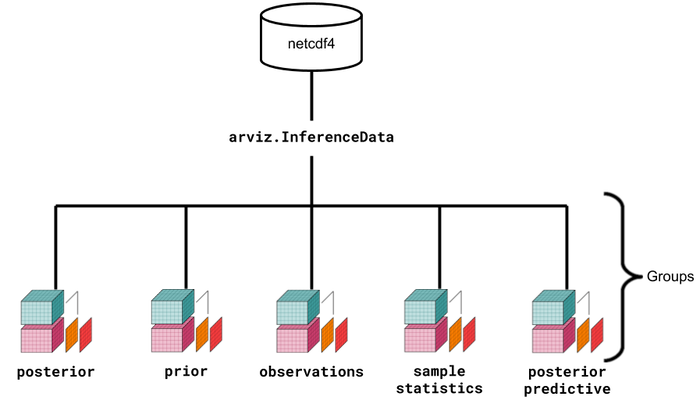
\includegraphics[width=0.6\linewidth]{InferenceDataStructure.png}
  \caption{Visual representation of \texttt{InferenceData}
  structure.}\label{fig:data}
\end{figure}

These groups are thought to contain a specific quantity such as \emph{posterior},
\emph{observed data} or \emph{sampler stats} (sampler quantities like
divergencies or tree depth, currently, the pointwise log likelihood is
stored here too). Groups in \texttt{InferenceData} directly translate to
groups defined in netCDF files, making the storage of \texttt{InferenceData}
objects in netCDF files straightforward. The full schema specification
can be found at ArviZ
documentation\footnote{\url{https://arviz-devs.github.io/arviz/schema/schema.html}}.

\texttt{InferenceData} objects are central to ArviZ, most of ArviZ functions
take \texttt{InferenceData} as input. Therefore, we provide native functions
to convert between the outputs of several inference libraries and
\texttt{InferenceData}. Table~\ref{tab:from_xyz} shows the state of
converter functions in ArviZ beta release 0.6.1 (latest release to date).
Currently supported libraries are PyStan, CmdStan and CmdStanPy
\cite{stan2018language, stan2018math, stan2018core, pystan2018}, % chktex 2
PyMC3~\cite{pymc32016}, Pyro and NumPyro~\cite{pyro2018},
emcee~\cite{emcee2013, emcee2019} and
TensorFlow Probability~\cite{tensorflow_probability2017}.

\begin{table}[!ht]
  \caption{ArviZ converter function summary}\label{tab:from_xyz}
  \begin{tabular}{ccccc}
    \toprule
    Inference Library&Sampler Stats&Posterior predictive&Observed data&Prior\\
    \midrule
    PyStan, CmdStan, CmdStanPy & \faCheck{} & \faCheck{} & \faCheck{} & \faCheck{} \\
    PyMC3 & \faCheck{} & \faCheck{} & \faCheck{} & \faCheck{} \\
    Pyro & \faCheck{}\footnote{For Pyro<1.0.0 there is only partial sampler
      stats support and no observed data available}
         & \faCheck{} & \faCheck\footnotemark[\value{footnote}] & \faCheck{} \\
    NumPyro & \faCheck{} & \faCheck{} & \faCheck{} & \faCheck{} \\
    emcee & Limited\footnote{emcee's blobs can be used to store sampler
    stats or even posterior predictive samples, however, blobs can store
  anything, so it is up to the user to customize them properly}
          & Limited\footnotemark[\value{footnote}]
          & \faCheck{} & \faTimes{} \\
    tensorflow probability & Limited\footnote{Only log likelihood data is
    retrieved} & \faCheck{} & \faCheck{} & \faTimes{} \\
  \bottomrule
\end{tabular}
\end{table}

All data currenlty stored in \texttt{InferenceData} is related to the Bayesian
inference run itself, either directly or indirectly. For example, posterior
predictive samples stored are intended for model checking and therefore do not
support predictions which would be out of sample posterior predictive samples.
We are still working in the \texttt{InferenceData} scheme in order to support
storage of predictions and to also store the arguments passed to the sampler
call as well as the kind of sampler.

\section{Statistics and diagnostics}\label{sec:stats}
ArviZ includes the most common statistics and diagnostics for Bayesian
analysis such as the Gelman-Rubin statistic~\cite{gelman1992rhat} or the
Watanabe-Akaike Information Criterion~\cite{watanabe2010waic}.
We strive to provide sensible default for all algorithms and to
keep them up to date with the latest publications. Moreover,
Numba~\cite{lam2015numba} is used to
speed up lengthy calculations.

\subsection{Diagnostics}
Many convergence assessment functions are available in ArviZ.
\texttt{az.rhat}, \texttt{az.ess} and \texttt{az.mcse}
implement the Gelman-Rubin statistic, effective sample size and Monte Carlo
Standard Error respectively \cite{gelman1992rhat, gelman2013bayesian}. % chktex 2
The improvements in \citet{vehtari2019rank} have already been added to
ArviZ and made the default for all 3 functions. Moreover, all 3 functions take
as input the method to be used for the calculation. For example, the effective
sample size can be calculated for the bulk or for quantiles and with or without
rank normalization. \texttt{az.bfmi} can be used to calculate Bayesian fraction
of missing information~\cite{betancourt2016diagnosing}. \texttt{az.geweke}
implements the z-scores for convergence diagnostics~\cite{geweke1991evaluating}.

An \texttt{az.summary} function is also provided for convenience to calculate
several diagnostics and statistics such as mean and variance at the same time.
Its output can be directly printed in a readable manner.

\subsection{Model comparison}
ArviZ also provides functions for model comparison using the predictive
accuracy as metric. Given that ArviZ is intended to analysis of Bayesian
inference results and it aims to extend best practices, only the fully
Bayesian algorithms have been implemented~\cite{gelman2014understanding}.
\texttt{az.waic} computes the
widely applicable information criterion~\cite{watanabe2010waic} and
\texttt{az.loo} computes the leave one out cross validation using Pareto
smoothed importance sampling~\cite{vehtari2015pareto, vehtari2017practical}.

\texttt{az.compare} can be used to compute the WAIC or LOO value for several
models at the same time, effectively comparing them in a single line of code.

\subsection{Model checking}
One algorithm for model checking, \texttt{az.loo\_pit}, has also been implemented
recently, the leave
one out cross validation pareto integrated transform
(LOO-PIT)~\cite{gabry2019visualization}. This has been possible thanks to the
versatility of \texttt{InferenceData}, which contains all the quantities
needed for this calculation: observed data, posterior predictive samples and
log likelihood data. It should be noted that the LOO-PIT result is generally
analyzed visually in a qualitative way, this can be also done in ArviZ using
native plotting functions. In addition, the results from \texttt{az.loo} and
\texttt{az.waic} can also be used for model checking to some extent.

\section{Data visualization}\label{sec:plots}
Many of the algorithms described in Section~\ref{sec:stats} have complemetary
plots that extend them and ease their interpretability. Some
examples are \texttt{az.plot\_compare}, \texttt{az.plot\_loo\_pit} or
\texttt{az.plot\_ess} which complement the algorithms of the same name, but
also \texttt{az.plot\_khat} to complement \texttt{az.loo} or
\texttt{az.plot\_elpd} to complement either \texttt{az.waic} or
\texttt{az.loo}.

ArviZ provides plotting functions suited for many different tasks:
visualization of probabiliy distributions, model checking, convergence
diagnostics or model comparison. The
documentation contains an
\href{https://arviz-devs.github.io/arviz/examples/index.html}{example gallery}
showcasing all plots currently available in ArviZ. Figure~\ref{fig:examples}
shows some of the recently added plots.

\begin{figure}[!htb]
\centering
  \begin{subfigure}{.47\textwidth}
  \centering
    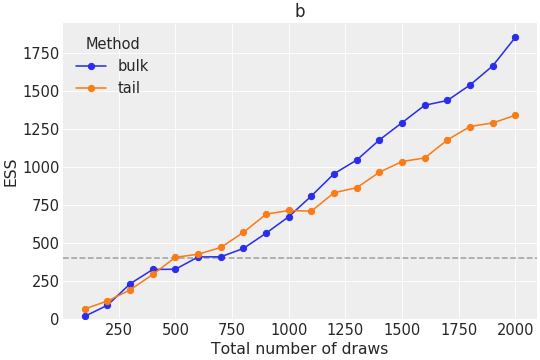
\includegraphics[width=\linewidth]{plot_ess.png}
    \caption{Evolution of the effective sample size as the sample size
    increases. A non-linear evolution of the effective sample size
    indicates convergence problems~\cite{vehtari2019rank}.}
  \end{subfigure}
  \begin{subfigure}{.47\textwidth}
  \centering
    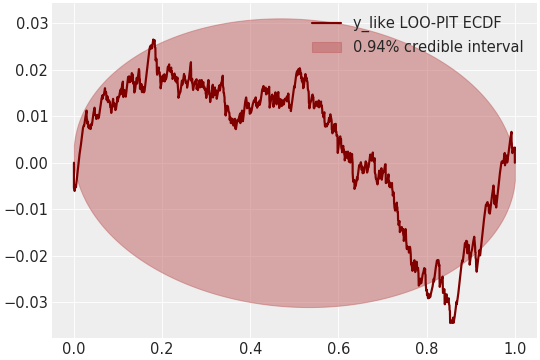
\includegraphics[width=\linewidth]{plot_loo_pit.png}
    \caption{LOO-PIT values estimated probabiliy density function. Differing
      from a uniform distribution indicates model
      mispecification~\cite{gabry2019visualization}.}
  \end{subfigure}\\
  \begin{subfigure}{0.98\textwidth}
  \centering
    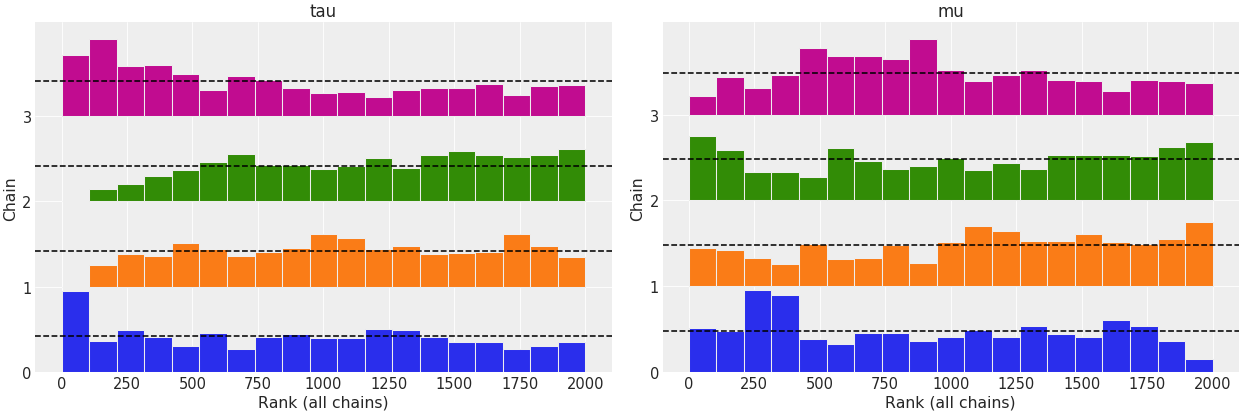
\includegraphics[width=\linewidth]{plot_rank.png}
    \caption{Rank plots are an alternative to the commonly used trace
      plots~\cite{vehtari2019rank}.}\label{fig:n2}
  \end{subfigure}
  \caption{Examples of plotting functions added to ArviZ during
  2019.}\label{fig:examples}
\end{figure}

\section*{Funding}
Work by Osvaldo Martin was supported by CONICET-Argentina and ANPCyT-Argentina
(PICT-0218). Two students were funded by the Google Summer of Code project to
work on ArviZ between May and August 2019.

\begin{acks}
  We would like to acknowledge all the comunities involved in ArviZ
  development ---especially Adrian Seyboldt, Junpeng Lao,
  Thomas Wiecki and Robert Goldman from the PyMC community, Allen Riddell and
  Aki Vehtari from the Stan community and Du Phan from the Pyro community.
  We also would like to thank everyone who contributed to ArviZ sending pull
  requests or posting issues, and the contributors of the libraries used to
  build ArviZ ---particularly xarray, matplotlib, bokeh and numpy.
\end{acks}

\bibliographystyle{acm-reference-format}
\bibliography{probprog-2020-proposal}

% \appendix
% \section{Appendices}

\end{document}
